\section{Eulerian Graphs and Circuit}

\begin{definition}[Eulerian Circuit]
    Given a graph $G = (V,E)$, an \textit{\textbf{Eulerian circuit}} is a sequence of vertices $x_0,\ldots,x_t$ such that
    \begin{itemize}
        \item $x_0 = x_t$ 
        \item $\forall i \in [t].\, \{x_i, x_{i+1}\} \in E$ 
        \item $\forall e \in E.\, \exists \text{ unique $i \in [t]$.}\, e = \{x_i, x_{i+1}\}$ (i.e. every edge appears exactly once in an Eulerian circuit)
    \end{itemize}
\end{definition}

We say a graph is \textit{\textbf{Eulerian}} if and only if it has an \textbf{Eulerian circuit}. An Eulerian circuit is also referred to as an \textbf{Euler tour} in some texts. The notion of an Eulerian circuit and graph appears in the famous problem of the \textbf{bridges of K\"onigsberg}.

In 1736, Euler gave his famous characterization of an Eulerian graph, stated as follows

\begin{theorem}[Euler, 1736]
    A connected graph $G = (V,E)$ is Eulerian if and only if all its vertices have even degree.
\end{theorem}

\begin{proof}
    The forward direction of the proof is quite straightforward whereas the reverse direction requires a slightly more involved proof by induction.

    ($\implies$): Let $G$ be a connected graph. Assume that $G$ is Eulerian so it must have an Eulerian circuit. Note that in an Eulerian circuit, every time we enter a vertex, we must also leave the vertex. This is the case for all vertices because otherwise we would have an infinite graph. Hence, all vertices in $G$ must have even degree.

    $(\impliedby)$: Let $G$ be a graph. We proceed by strong induction on the number of edges.

    \textbf{Base Case}: $G$ is a graph with $m = 0$ edge. The result trivially holds.

    \textbf{Inductive Step}: Let $m \in \N$ be arbitrary. Assume that for all $k \in \N$ such that $0 \leq k < m$, the implication holds. Let $G = (V,E)$ be a connected graph with $m$ edges. Further, assume that $\deg_G(v)$ is even for all $v \in V$. Since the graph is connected and every vertex has even degree, it follows immediately that $\deg_G(v) \geq 2$ for all $v \in V$. This also implies that $G$ contains a cycle. Let $c = v_1\ldots v_k$ be such cycle of maximal length and $E'$ be the edges contained in this cycle.

    If $c$ contains all edges exactly once, we are done. Hence, suppose $E' \neq E$ and consider the graph $G' = (V, E \setminus E')$. It has connected components $S_1, \ldots, S_l$. Since $E' \neq E$, each of the connected components $S_i$ contains strictly fewer edges than $|E| = m$. For every $v \in G$, an even number of edges of $G$ at $v$ are in the cycle $c$, so we we remove these edges, each vertex in the remaining graph should still have even degree. Apply the induction hypothesis to the components, which asserts that each of the components $S_1, \ldots, S_l$ possess an Eulerian circuit. Further, since $c$ is a cycle, $C = (\{v_1,\ldots,v_k\}, E')$ itself is also Eulerian. Now, we recursively construct an Eulerian circuit, say $x$, in the original graph $G$. Start from $v_1$, find the component $S_i$ containing $v_1$, and concatenate the Eulerian tour in $S_i$ to $x$. Next, move from $v_1$ to $v_2$ along $\{v_1,v_2\} \in E'$. If $\{v_1,v_2\} \not\in E$, then they must have been in the same connected component, in which case we skip $v_2$ and move to $v_3$. Repeat this until we have walked through every edge in each one of the $l$ connected components and the edges in $E'$ connecting each component. It is clear that $x$ is Eulerian since it visits every edge exactly once.

    By induction, the implication holds.
\end{proof}

\begin{figure}[htbp]
    \centering
    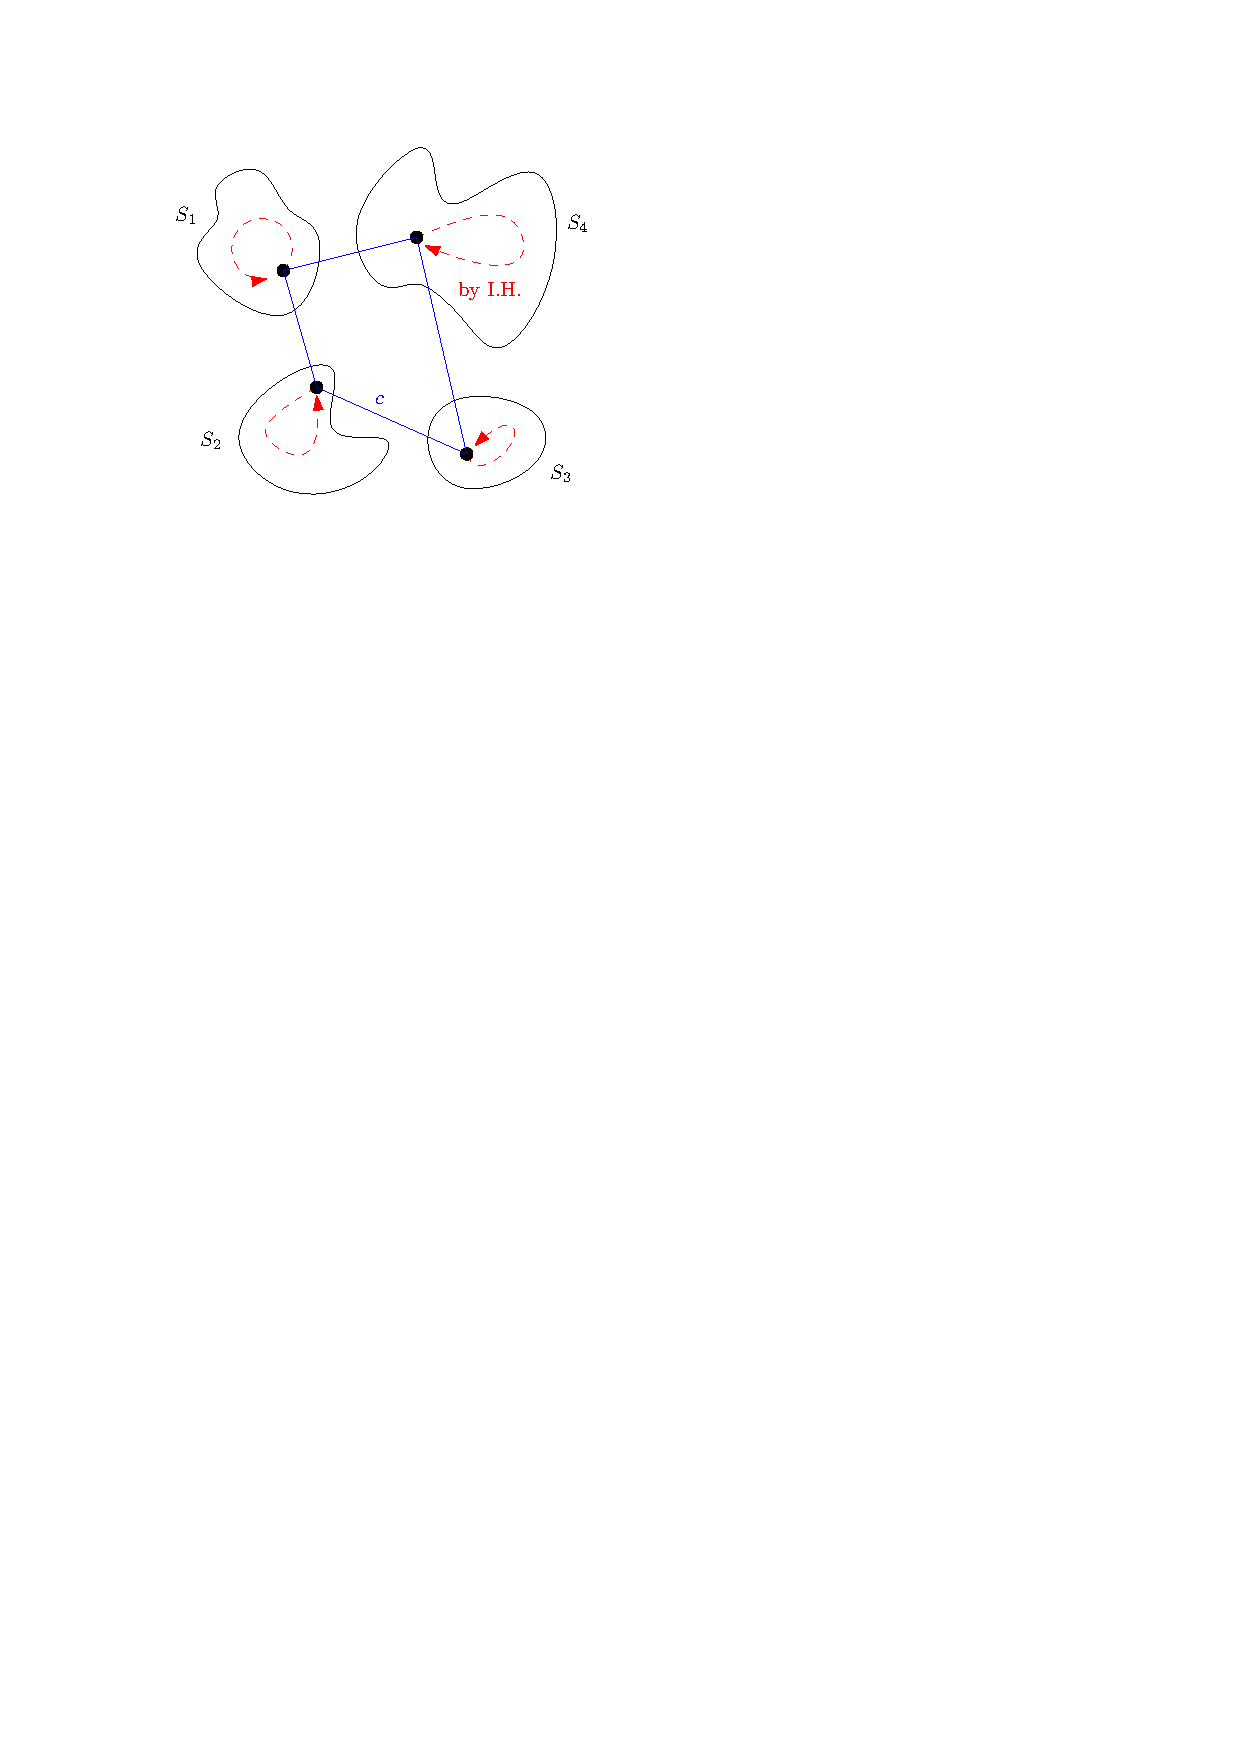
\includegraphics[width=0.3\linewidth]{figures/eulerian-circuit-construct.pdf}
    \caption{Construct an Eulerian circuit in the original graph $G$ by first finding a cycle $c$, remove the cycle, find an Eulerian circuit within each component $S_1,\ldots,S_l$, and concatenate these circuits via the cycle $c$.}
    \label{fig:euler-circuit-construct}
\end{figure}

\section{Hamiltonian Graphs}

\begin{definition}[Circuits]
    A \textit{\textbf{circuit}} in a graph $G = (V,E)$ is a sequence of distinct vertices $v_1,\ldots,v_k$ such that for all $i \in \{1,\ldots, k-1\}$, $\{v_i,v_{i+1}\} \in E$ and $\{v_k,v_1\} \in E$. Note, a circuit induces a copy of a subgraph isomorphic to $C_k$ for $k \geq 3$. Specially, we define a \textbf{single vertex} a circuit as well.
\end{definition}

\begin{definition}[Hamiltonian Graph]
    We call a graph with $n$ vertices \textit{\textbf{Hamiltonian}} if it admits a circuit of length $n$, which is to say that the graph has a spanning subgraph that is isomorphic to $C_n$.
\end{definition}

A sufficient condition for Hamiltonian graphs.

\begin{theorem}[Dirac, 1952]
    Let $G = (V,E)$ be a graph with $n$ vertices where $n \geq 3$. Suppose that for every $v \in V$, $\deg_G(v) \geq \ceil{\frac{n}{2}}$. Then, $G$ is Hamiltonian.
\end{theorem}

\begin{proof}
    Let $G = (V,E)$ be a graph with $n \geq 3$ vertices. Assume that $\deg_G(v) \geq \ceil{\frac{n}{2}}$ for all $v \in V$. Let $\delta(G)$ denote the minimum degree. That is, $\delta(G) = \min \{\deg_G(v) \mid v \in V\}$. Then, the assumption is equivalent to that $\delta(G) \geq \ceil{\frac{n}{2}}$.
    
    We claim that $G$ is connected. We prove the claim by contradiction. So suppose not, consider the component $G' = (V_{G'}, E_{G'})$ of $G$ with the fewest number of vertices. Since $\delta(G) \geq \ceil{\frac{n}{2}}$, each vertex is connected to at least $\ceil{\frac{n}{2}}$ other vertices. Since $C$ is a component that is not connected to vertices in other components, $|V_{G'}| \leq \ceil{\frac{n}{2}}$. But then, $\delta(G') < |V_C| \leq \ceil{\frac{n}{2}}$, which contradicts the assumption that $\deg_G(v) \geq \ceil{\frac{n}{2}}$ for all $v \in V$, including those in $G'$.

    Since $G$ is connected, we can find the longest path in $G$. Let $P = v_0 \ldots v_k$ be a longest path in $G$ of length $k$ (with $k$ edges and $k+1$ vertices). We claim that there exists some $0 \leq i \leq k-1$ such that $\{v_0,v_{i+1}\} \in E$, $\{v_i, v_k\} \in E$, and $\{v_i, v_{i+1}\} \in E$ as shown in Figure \ref{fig:dirac-thm-path}.

    \begin{figure}[htbp]
        \centering
        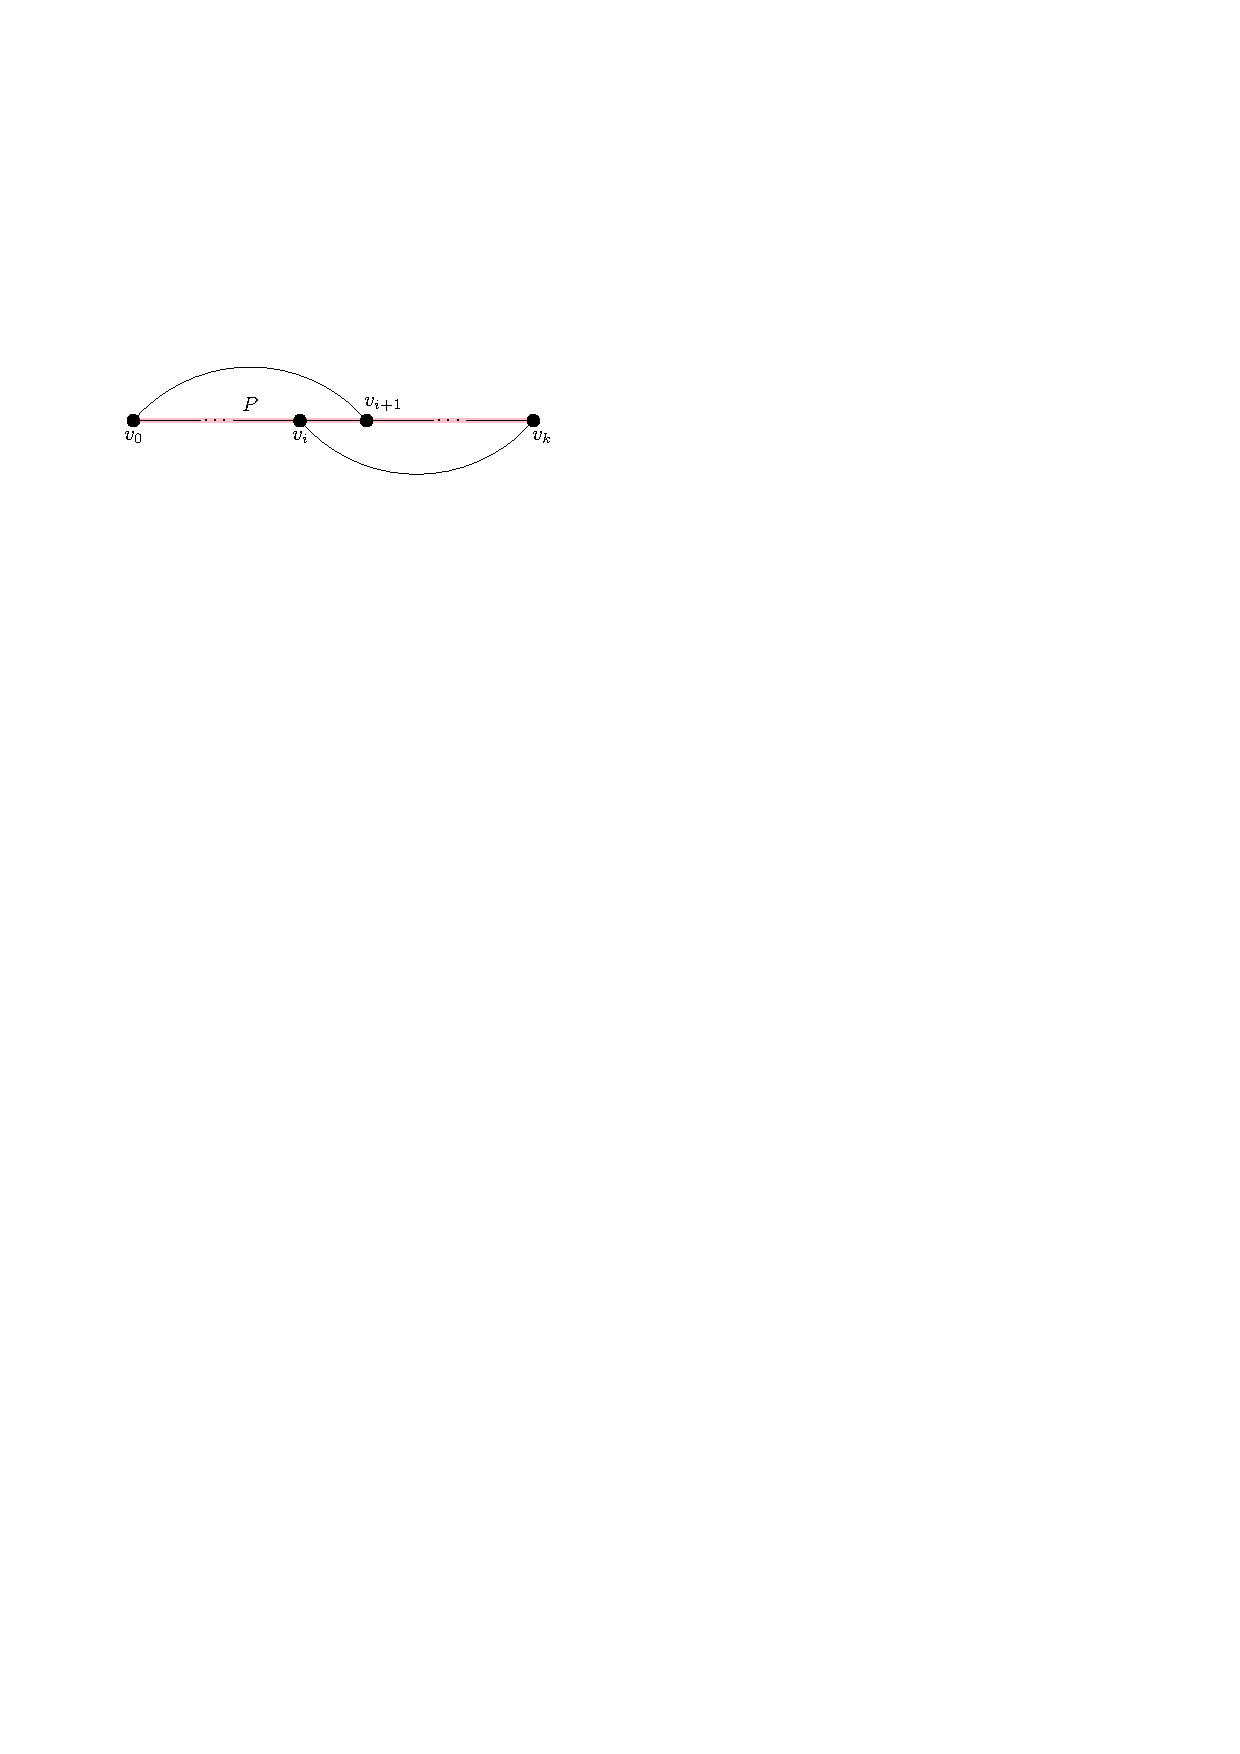
\includegraphics[width=0.4\linewidth]{figures/dirac-thm-path.pdf}
        \caption{The longest path $P = v_0\ldots v_k$ with $k+1$ vertices is colored in red. There exists some $0 \leq i \leq k$ such that $\{v_0,v_{i+1}\} \in E$ and $\{v_i,v_k\} \in E$.}
        \label{fig:dirac-thm-path}
    \end{figure}

    Such adjacent vertices $v_i$ and $v_{i+1}$ such that $v_i$ is adjacent to $v_k$ and $v_{i+1}$ is adjacent to $v_0$ must exists. By way of contradiction, suppose $v_i$ and $v_{i+1}$ do not exist. Then, for every vertex adjacent to $v_0$, there must exists some vertex adjacent to it that is NOT adjacent to $v_k$. Similarly, for every vertex adjacent to $v_k$, there must exists some adjacent vertex that is NOT adjacent to $v_0$. Note that these two sets of vertices are disjoint and do not include $v_k$. This implies that
    $$
    \deg_G(v_0) + \deg_G(v_k) + 1 \leq k + 1
    $$
    since we are not overcounting and the number of vertices being counted is at most the length of path $P$. The additional 1 on the LHS of the inequality came from couting $v_k$ as it is not included in either $\deg_G(v_0)$ or $\deg_G(v_k)$. Now, since $\deg_G(v) \leq \ceil{\frac{n}{2}}$ for all $v \in V$,
    $$
    n + 1 \leq \left\lceil \frac{n}{2} \right\rceil + \left\lceil \frac{n}{2} \right\rceil + 1 \leq \deg_G(v_0) + \deg_G(v_k) + 1 \leq k + 1
    $$
    so $n + 1 \leq k+1$. This implies that $n < k+1$ since both $n$ and $k$ are integers. But this leads to a contradiction because the number of vertices on the path $P$ cannot be more than the total number of vertices in the entire graph.

    The existence of such $v_i$ and $v_{i+1}$ allows us to construct a cycle $C = v_0 \to v_{i+1} \leadsto_{P} v_k \to v_i \leadsto_{P} v_0$. We claim this cycle is Hamiltonian.

    \begin{figure}[htbp]
        \centering
        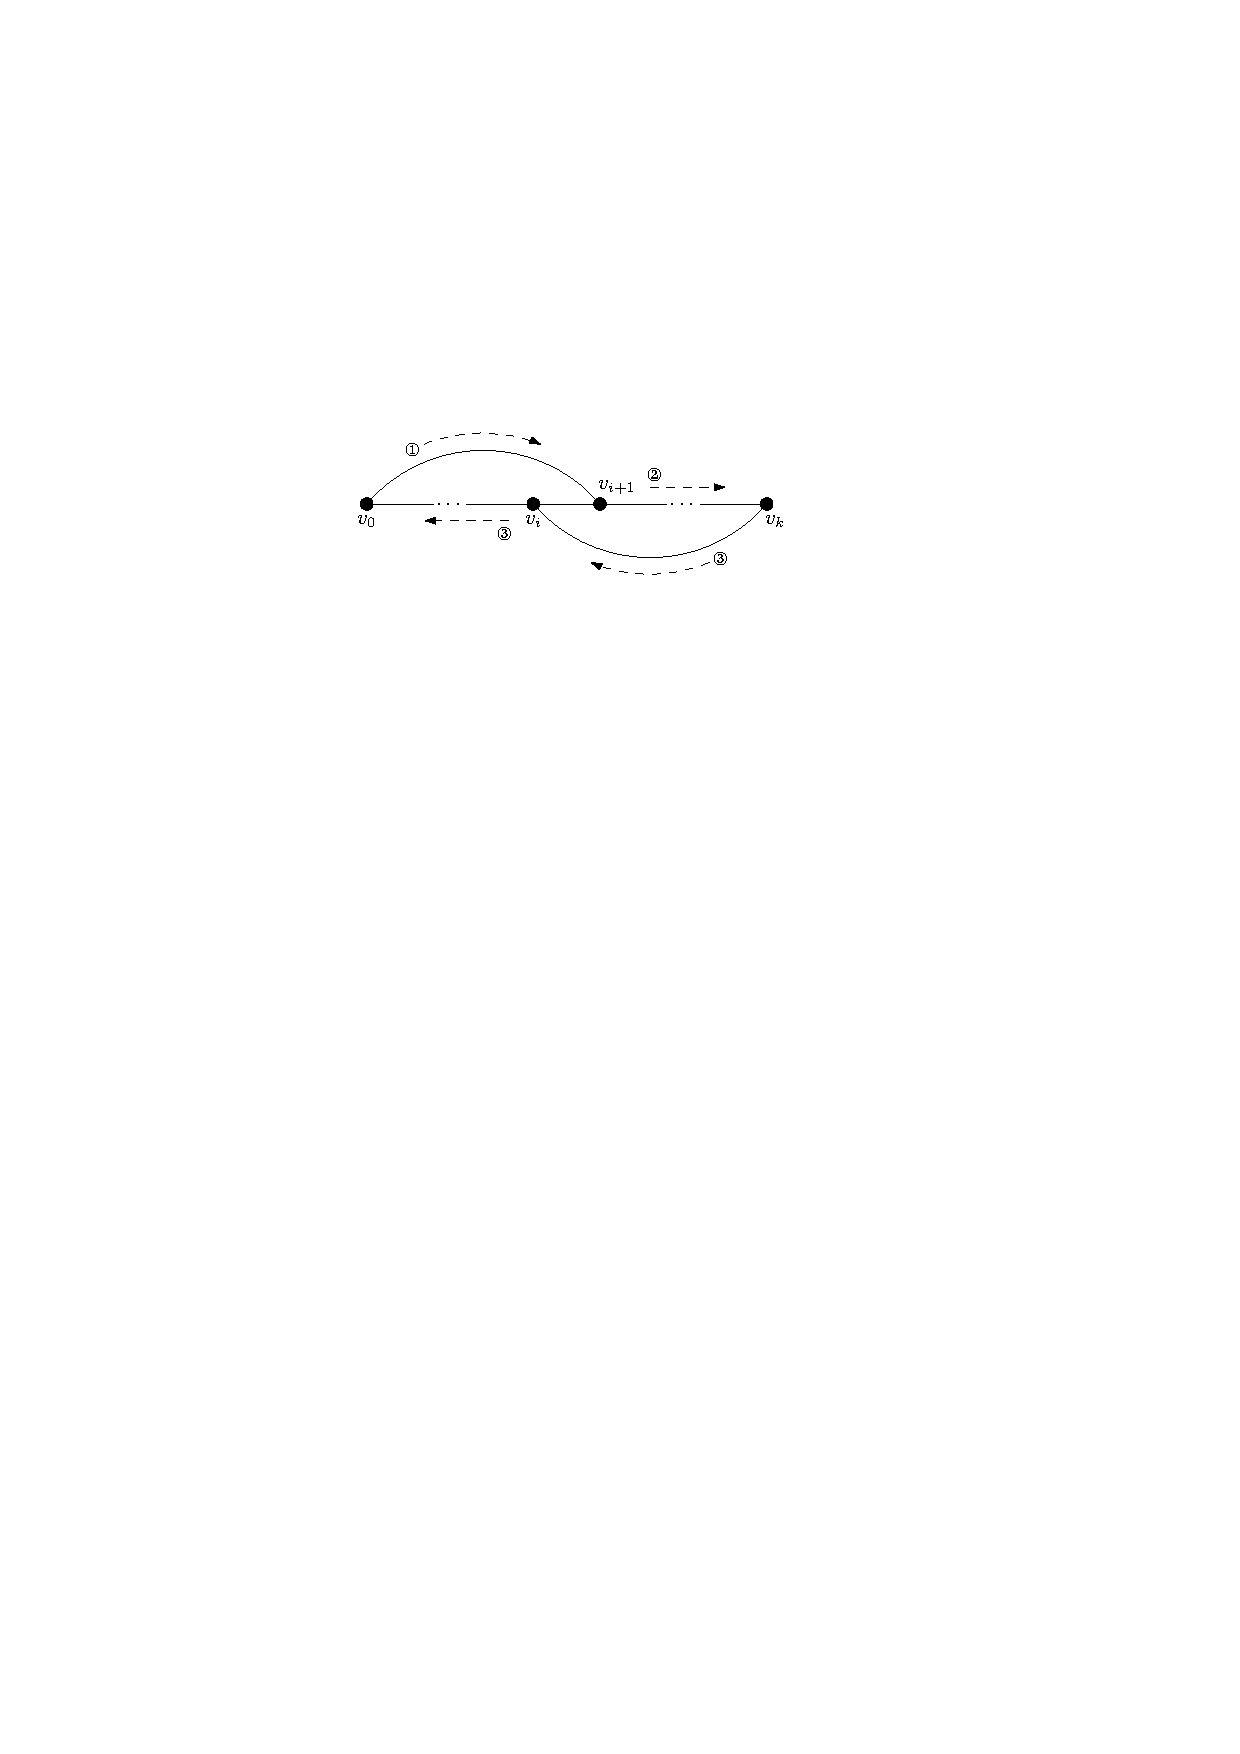
\includegraphics[width=0.4\linewidth]{figures/dirac-thm-hamcycle.pdf}
        \caption{The Hamiltonian path is $C = v_0 \to v_{i+1} \leadsto_{P} v_k \to v_i \leadsto_{P} v_0$.}
        \label{fig:dirac-thm-hamcycle}
    \end{figure}

    To see why $C$ is Hamiltonian, again we use a contradiction proof. Suppose $C$ is not Hamiltonian. Then, by definition, there must be some vertex $w \in V$ such that $w$ is not on $C$. But since $G$ is connected, $w$ must be adjacent to some vertices, say $v_w \in V$. Without loss of generality, suppose that this $v_w$ is on the cycle $C$. There must also be a $v_{w+1}$ immediately adjacent to $v_w$. By construction, the cycle $C$ contains $k+1$ edges (that's all edges on $P$ along with $\{v_0,v_{i+1}\}, \{v_i,v_k\}$ and without $\{v_i,v_{i+1}\}$). We then consider the path from $v_w$ to $v_{w+1}$ by following the edges on the cycle. This leads to a path of length $k$, namely $p = v_w \leadsto v_0 \to v_{i+1} \leadsto v_k \to v_i \leadsto v_{w+1}$. Now, we extend the left end of this path to $w$ since $w$ is adjacent to $v_w$ and still get back a valid path. The new path $P' = w \to v_w \leadsto v_0 \to v_{i+1} \leadsto v_k \to v_i \leadsto v_{w+1}$ is one edge longer than $p$. However, this contradicts the maximality assumption for $P$ since now we would have a path, $P'$, that contains more vertices than $P$. Therefore, $C$ is indeed a Hamiltonian path.

    \begin{figure}[htbp]
        \centering
        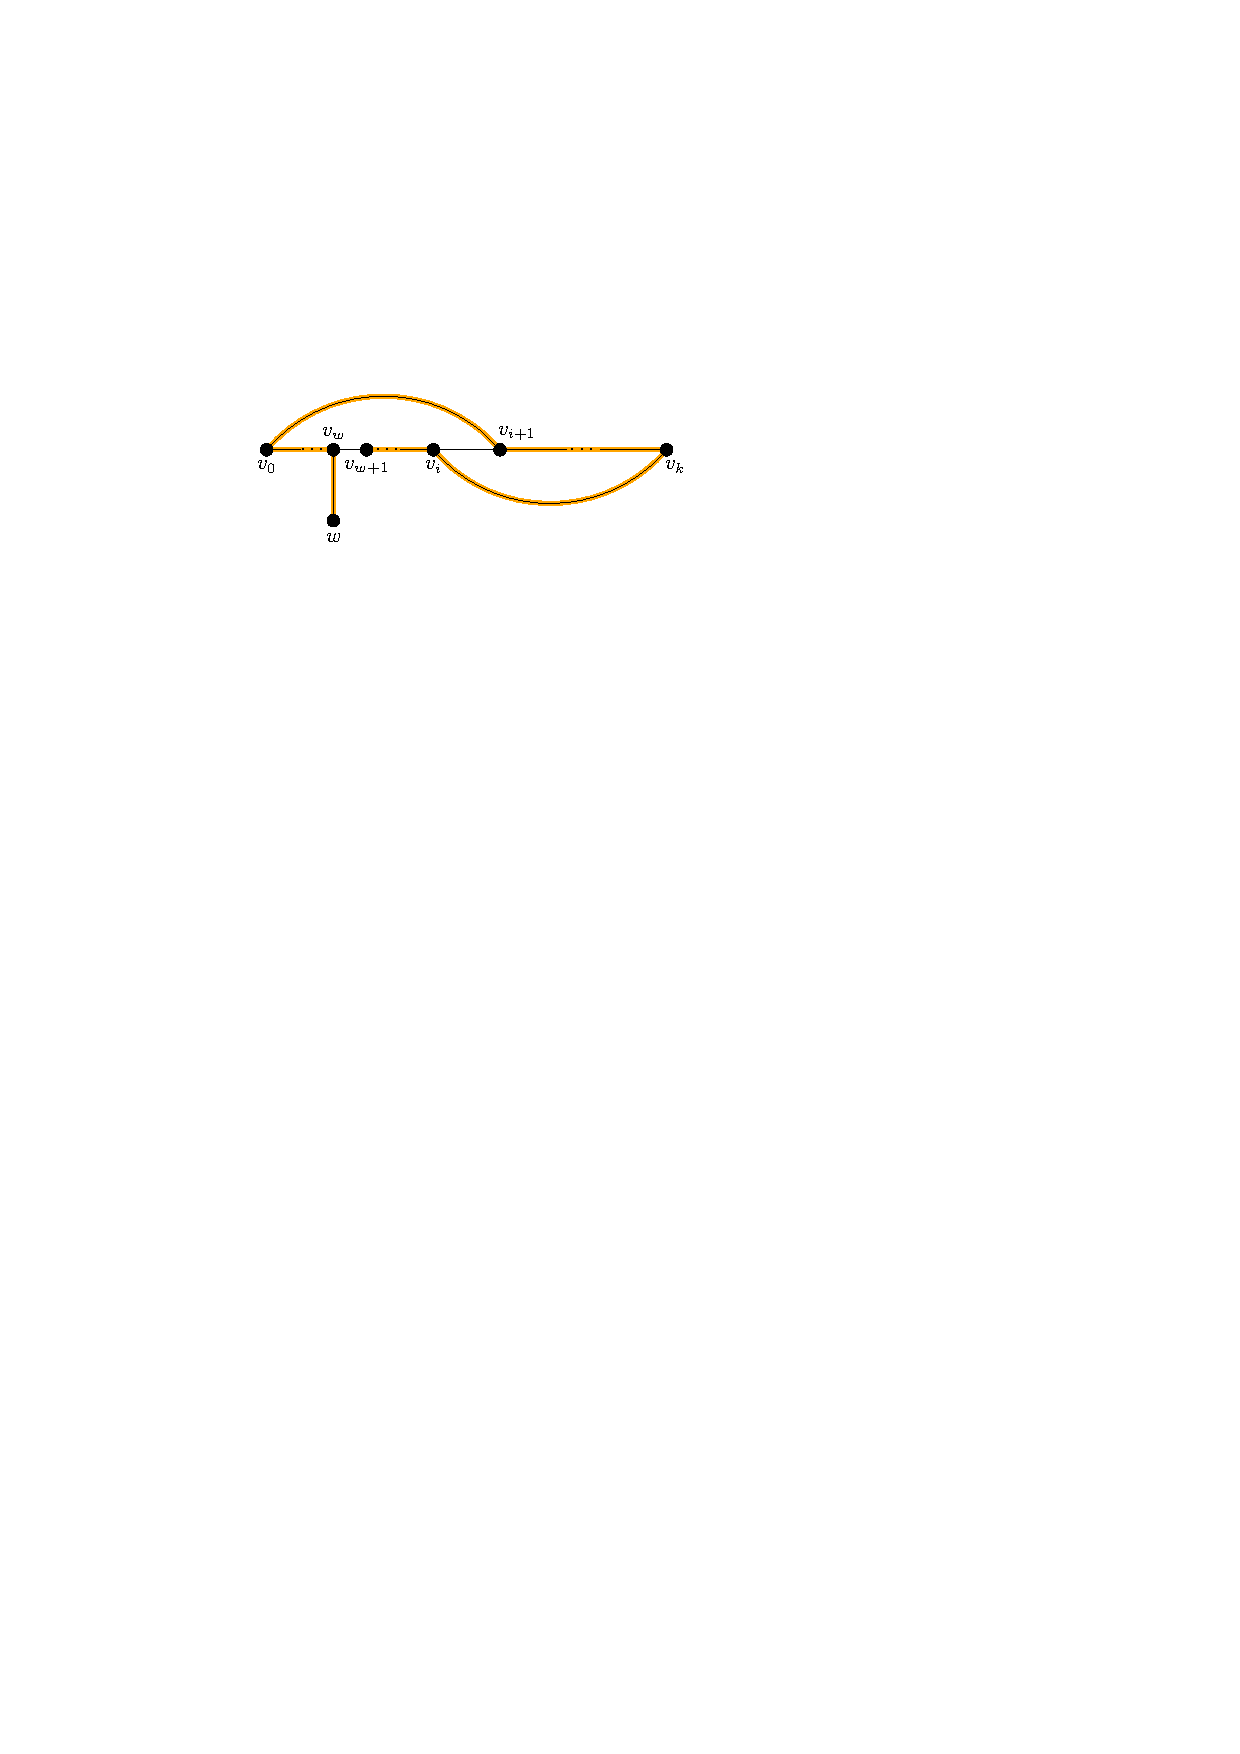
\includegraphics[width=0.4\linewidth]{figures/dirac-thm-longer-path-contradiction.pdf}
        \caption{With the existence of a vertex $w$ outside of the previously constructed cycle, we would have a longer path (colored in orange), contradicting the maximality of $P$.}
        \label{fig:dirac-thm-path-contradiction}
    \end{figure}

    It follows immediately that $G$ is Hamiltonian by definition.
\end{proof}